%-----------------------------------------------------------------------
\subsection{DMI Controller}
%-----------------------------------------------------------------------
%\tbc
%Valerio D´Angelo/Baseliyos Jacob

\paragraph{Reference to the SRS or other Requirements (or other requirements)}

§ 4.7, § 5.4, § 3.12.3

\subparagraph{§ F I1: Packet 72:} this packet will inclsude the information received from the track for the entered section with the display and display conditions depending from:\\
  - train status Level ETCS\\
  - train status modus ETCS\\
  - distance\\
  - timeperiod\\
  - acknowledgement from the driver on the DMI display\\
The displaying of this information can be ordinary or multiple (combination of several conditions). \\

\subparagraph{§ F I2: Missing acknowledgement:}
for the case that a acknowledgement from the driver in combination with another condition is expected at the end, and the acknowledge is missing, the ETCS on-board unit will trigger the service brake.(missing acknowledgement).\\

\subparagraph{§ F I3: Packet 76:} this package contains information for sending fixed messages. \\

\paragraph{Short descriptoiin of the functionality}
The DMI controller interact with the DMI display and is responsible for alls procedures between the DMI display and Driver. Furthermore the DMI controller will interact with the DMI Management to compute the receive information (e.g. driver number request, ...) and send, if necessary, data or reports ot the DMI Management (acknowledge, text messages, ..).\\

\begin{figure}[hbtp]
\centering
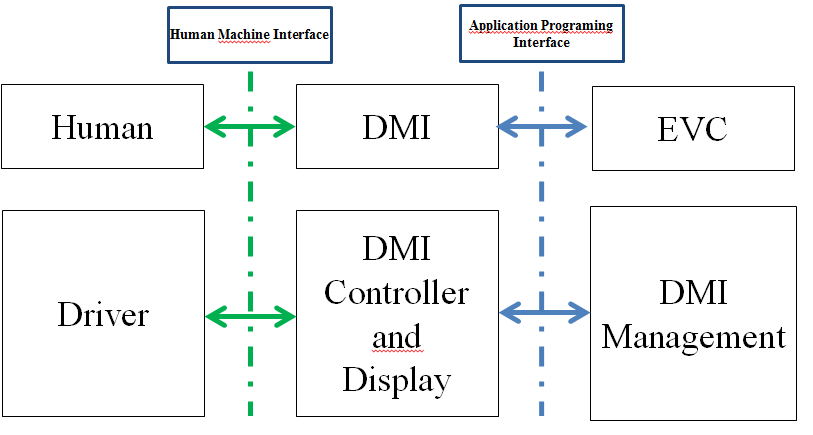
\includegraphics[scale=0.5]{images/DMI_Interfaces}
\caption{DMI Interfaces}
\end{figure}

\paragraph{Interface}

\paragraph{Functional Design Description}

\paragraph{Refernce to the Scade Model}

\textbf{only in special case or link to the Scade model}

